



\textbf{Setup}. There is a Wi-Fi AP and client pair. The received Wi-Fi power at the 
client is -45dBm, if the maximum transmission power is used. 
The LTE-U base station is put at the middle of the Wi-Fi AP
and the client, so that both AP and client can receive the same level of interference
caused by LTE-U base station. 
To emulate different distances from LTE-U base station to Wi-Fi AP and client,
We use two laptops as the UDP server and UDP client, respectively. 
The UDP server connects with the Wi-Fi AP with ethernet cable. 
we vary the transmit power of LTE-U base station. 
We use iperf software package to setup a UDP link between Wi-Fi AP and client. 
The interference-free UDP throughput of the Wi-Fi link is around 95Mbps.
Each iperf round is 30s UDP throughput measurement. 
For each setting, we measure 10 rounds of iperf throughput tests. 
We assume symmetric transmit power and attenuation between LTE-U base station
and Wi-Fi AP, i.e., if the received Wi-Fi power is -62dBm at the 
LTE-U base station, the received LTE-U power is also -62dBm at the Wi-Fi AP. 



\textbf{Wi-Fi Routers}. 
We use three different routers installed with various firmwares to represent
commerial router, DD-WRT router \cite{ddwrt} and OpenWRT router \cite{openwrt}. 
The commerial router is TP-Link WR940N. 
We installed DD-WRT on Buffalo N900 and 
installed OpenWRT on NetGear N600 WNDR3700v4.
Ideally we want to measure different firmwares on the same 
device and the hardware difference can be eliminated. 
But DD-WRT and OpenWRT do not support all the devices
and we find no overlapped device that is 
compatible with both firmwares under 802.11n protocol.
Unless otherwise specified, the routers run the default rate-adaptation algorithms. 



\textbf{Methodology}.
We vary several LTE-U parameters and evaluate the interference
to the three different Wi-Fi routers. 
The first one is the level of the interfering LTE signal observed at the AP. 
This is currently also used as a proxy for the RSSI of WiFi signal measured at the eNodeB when carrier sensing, 
since the channel is typically symmetric (we will implement accurate measurement in future). The second one is the LTE traffic load. The third one is LTE-U duty cycle. 
It is important to emphasize the difference between the traffic load and duty cycle. 
Even when there is no traffic, an ordinary LTE keeps sending reference signals which cause interference to WiFi. 
In order to reduce interference, LTE-U defines duty cycle. 
In the ``off'' part of the cycle LTE-U is completely idle 
and doesn't create any interference to WiFi (it also ceases to transmit reference signals).



\begin{figure}[t] \centering 
    \begin{subfigure}[b]{\linewidth} \centering
     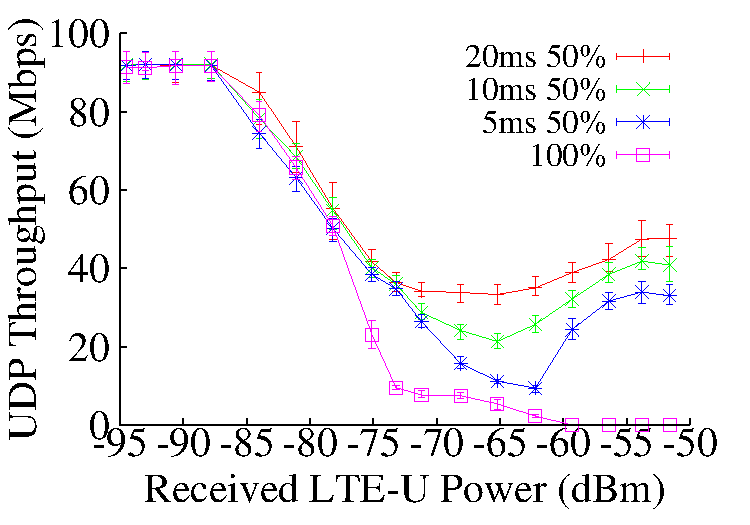
\includegraphics[width=3.0in, angle=0]{./figures/impact_power_tplink} 
         \vspace{-0.0cm}
         \caption{LTE-U interference on TP-Link WR940N, and we observe similar trend for Buffalo N900 installed with DD-WRT.}         
        \label{impact_power:a}
    \end{subfigure} %

    \begin{subfigure}[b]{\linewidth}  \centering 
     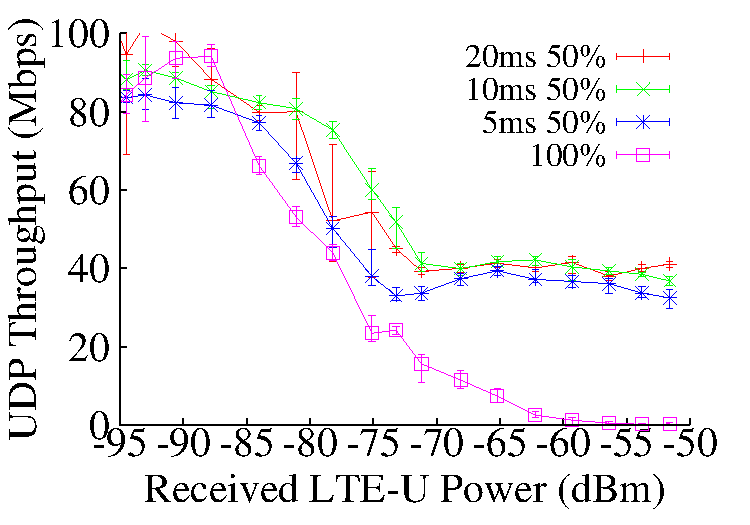
\includegraphics[width=3.0in, angle=0]{./figures/impact_power_openwrt}  
        \vspace{-0.0cm}
        \caption{LTE-U interference on NetGear N600 WNDR3700v4 installed with OpenWRT.}
        \label{impact_power:b}    
    \end{subfigure} 
\caption{The impact of various powers and ``on'' periods of LTE-U on three different kinds of Wi-Fi routers.}
\label{impact_power}
\vspace{-0.2cm}
\end{figure}


\begin{figure}[t] \centering
    \begin{subfigure}[b]{\linewidth} \centering
     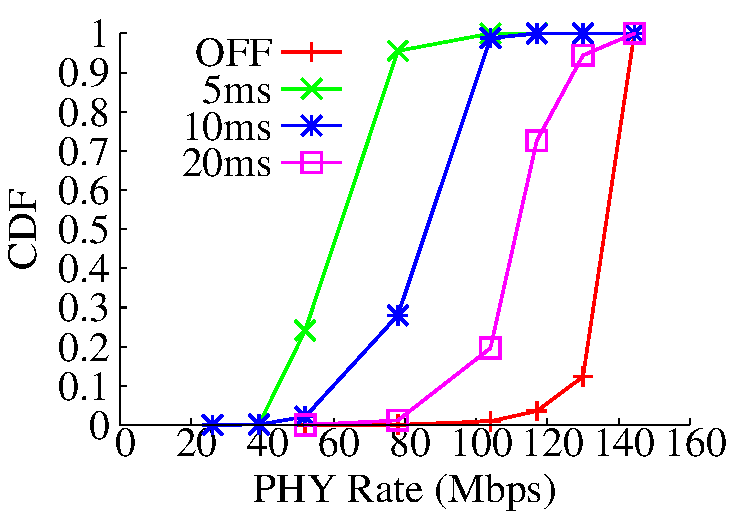
\includegraphics[width=3.0in, angle=0]{./figures/impact_ratecdf_tplink} 
         \vspace{-0.0cm}
         \caption{Wi-Fi PHY rates used by commerical router under 50\% duty cycle of LTE-U.}         
        \label{impact_cdfrate:a}
    \end{subfigure} %

    \begin{subfigure}[b]{\linewidth} \centering 
     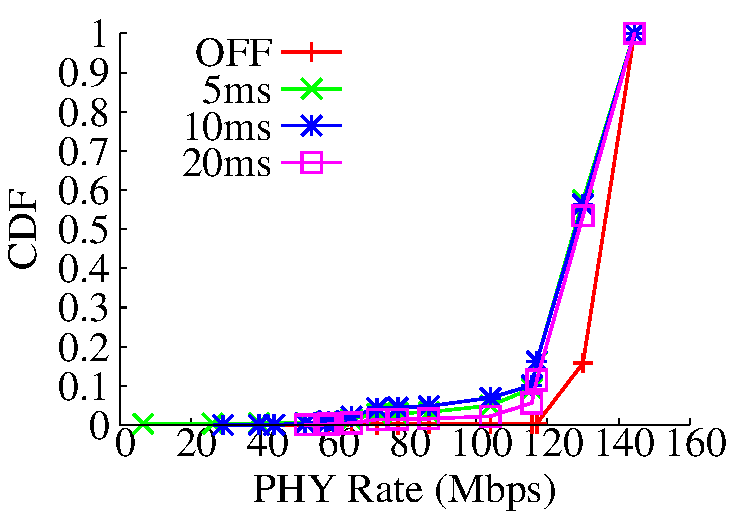
\includegraphics[width=3.0in, angle=0]{./figures/impact_ratecdf_openwrt}  
        \vspace{-0.0cm}
        \caption{Wi-Fi PHY rates used by OpenWRT under 50\% duty cycle of LTE-U.}
        \label{impact_cdfrate:b}    
    \end{subfigure} 
\caption{The PHY rates of different routers used under same interference settings.}
\label{impact_cdfrate}
\vspace{-0.2cm}
\end{figure}




\subsection{Sensing Threshold}


The LTE-U forum regulates that the LTE-U station is required to sense the energy level
to adjust duty cycle. 
The energy detection threshold is set to be -62dBm, 
which is the energy detection threshold in 802.11a/b/g/n standards. 
According to our measurement results, as shown in Fig. \ref{impact_power},
LTE-U may interfere with some routers even the 
received power at the Wi-Fi side is below the energy detection threshold.
In this measreument, 
the LTE-U base station broadcasts LTE signals in $100\%$ and $50\%$ duty cycles, respectively. 
For $50\%$ duty cycle, we use three different ``on'' time, 5ms, 10ms and 20ms.
It shows different interference pattern for two different routers. 



\textbf{Observations}.
For commercial router, as shown in Fig. \ref{impact_power:a},
the interference from LTE-U base station affects Wi-Fi UDP throughput dramatically 
at -75dBm. 
If the energy detection of LTE-U base station is set to be -62dBm, 
the LTE-U base station will send in $100\%$ duty cycle when there is
only one Wi-Fi link with sensed power below -62dBm. 
Wi-Fi can only maintain $10\%$ of interference-free throughput at -70dBm, 
which indicates Wi-Fi link is close to starving when 
LTE-U optimistically set the energy detection threshold to be -62dBm. 
At the meanwhile, the interference from LTE-U base station affects 
Wi-Fi throughput even when the LTE-U base station operates at $50\%$
duty cycle. 
The UDP throughput of Wi-Fi at 20ms ``on'' time is higher
than that at 5ms ``on'' time. 
We focus on received power in this section and leave the discussion of different ``on'' time
in later sections. 
For OpenWRT router, as shown in Fig. \ref{impact_power:b},
the interference from LTE-U base station affects Wi-Fi UDP throughput 
similarly when the received power is higher than -75dBm. 


\textbf{Reason}.
To examine why different routers show different performance 
on handling LTE-U interference,
we collected the Wi-Fi packets in the air by using 
a separated Wi-Fi monitor interface.
The data is collected when the received LTE-U power is around -75dBm. 
We examine the PHY rate used by commercial router
and OpenWRT router, and the results
are shown in Fig. \ref{impact_cdfrate}.
The CDF of commercial router PHY rates is plotted
in Fig. \ref{impact_cdfrate:a} and that of OpenWRT
router PHY rates is plotted in Fig. \ref{impact_cdfrate:b}. 
The PHY rate of commercial router is affected significantly
by LTE-U transmissions.  
Since the Wi-Fi router cannot sense the transmission of the
LTE-U, it concludes the dropped packets are caused
by channel condition instead of the collision.
It tried to lower the PHY rate and hope the 
lower rate packets can go through. 
It keeps doing that until reaches the lowest PHY rate.
OpenWRT is able to identify the packet drops (during LTE-U ``on'' time)
are caused by collision instead of signal attenuation.  



\begin{figure}[!ht]
 \centering
    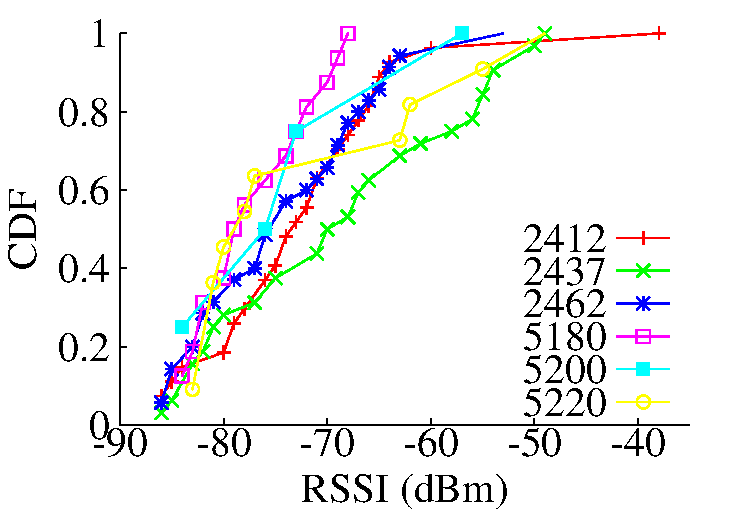
\includegraphics[width=0.4\textwidth]{./figures/public_ap_rssi}
 \caption{The RSSI distribution of public Wi-Fi APs.}
  \label{fig:public_ap_rssi}
\end{figure}



\textbf{Potential Impact to Public Wi-Fi}.
Considering that LTE-U signal may affect some of the
commercial routers, we want to understand how many
Wi-Fi networks could be interferenced once
LTE-U base stations are deployed. 
We study the public Wi-Fi characteristics using the traces collected 
from a shopping mall. 
The traces are collected in a coffee shop at Saturday 4pm. 
We create a monitor interface on a laptop and use \emph{libpcap}
library to capture the Wi-Fi data packets. 
We capture data packets from three channels in 2.4GHz 
(with center frequency 2412MHz, 2437MHz and 2462MHz) and
three channels from 5GHz (with center frequency 5180MHz, 5200MHz and 5220MHz), respectively. 
We collect 20 mins data traces from each channel. 
We repeat the same process in an apartment in a 
resident area and an office environments.
The Wi-Fi APs are identified if it broadcasts 
beacons to surrounding Wi-Fi clients. 
As shown in Fig. \ref{fig:public_ap_rssi}, 
the received power of more than 80\% of the APs 
fall between -80dBm to -62dBm, 
which could be sensitive to LTE-U interference, 
i.e., if we replace the Wi-Fi monitor 
with a LTE-U base station. 






\subsection{Duty Cycles and ``On'' Period}



In this experiment, we test if LTE-U duty-cycling is fair to Wi-Fi. 
We use two LTE-U power settings and the received LTE-U power at
the AP/client is -55dBm (above Wi-Fi energy detection threshold) 
and -70dBm (below Wi-Fi energy detection threshold), respectively.  
We use three on time cycles, 5ms, 10ms and 20ms. 
For each on time, we vary the duty cycle from $10\%$ to $90\%$. 
The results are summarized in Fig. \ref{impact_ontime}.

Because the LTE-U base station is not sensing Wi-Fi transmission
if the received power is under -62dBm, 
the starting of LTE-U on period may kill the Wi-Fi packet. 
Under the same duty cycle, say 50\%, 
the smaller the ``on'' period, the more Wi-Fi packets
are interferenced.
The drop of the Wi-Fi packet may trigger the Wi-Fi
rate adaptation algorithm to reduce the transmission rate. 
 

\begin{figure}[t] \centering
    \begin{subfigure}[b]{\linewidth} \centering
     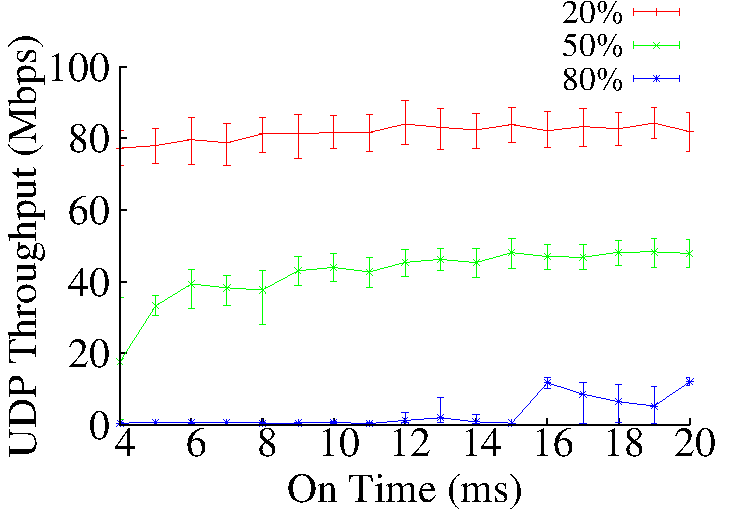
\includegraphics[width=3.0in, angle=0]{./figures/impact_ontime_tplink_above} 
         \vspace{-0.0cm}
         \caption{Received LTE-U power is above -62dBm.}         
        \label{impact_ontime:a}
    \end{subfigure} %

    \begin{subfigure}[b]{\linewidth} \centering 
     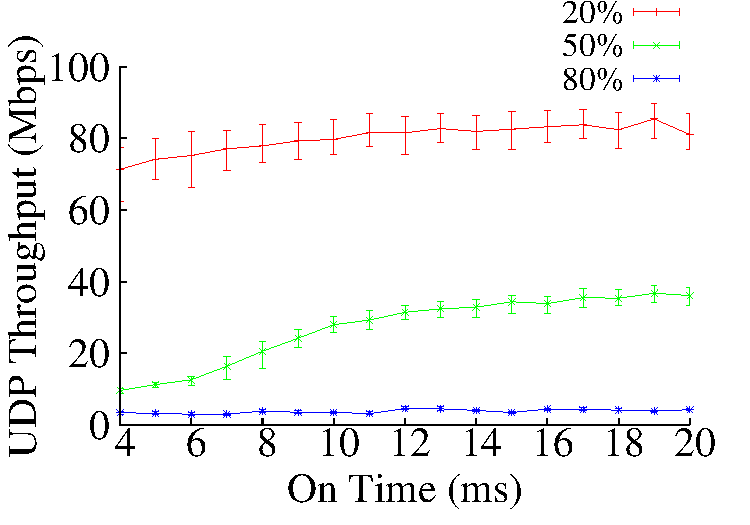
\includegraphics[width=3.0in, angle=0]{./figures/impact_ontime_tplink_below}  
        \vspace{-0.0cm}
        \caption{Received LTE-U power is below -62dBm.}
        \label{impact_ontime:b}    
    \end{subfigure} 
\caption{Impact of various LTE-U on periods and duty cycles.}
\label{impact_ontime}
\vspace{-0.2cm}
\end{figure}







\subsection{Number of Resource Blocks}


Each LTE frame consists of 10 subframes and the airtime of
each subframe is 1ms. 
In frequency domain, each subframe consists of many resource
blocks (RBs), e.g., a 20MHz LTE frame consists of 100 RBs.
LTE is transmitting synchronization signals by using some of 
the resource blocks even there is no data transmission. 
In this measurement, we want to check the impact of 
varied resource blocks. 
We fill the LTE frames with random data and use
the default setup. 
Different from previous measurements, 
we record LTE-U transmission power instead of received 
power at the Wi-Fi AP/client side. 
This is because the received power at the Wi-Fi side
varies to the number of resource blocks. 
Considering a deployed LTE-U base station, the transmission 
power is fixed, but the received interference signals
at the Wi-Fi side is different if the number of
resource blocks is different. 
We adjust the transmission power of the LTE-U base
station and show the impacts in Fig. \ref{impact_nrbs}.

The commercial router, which is more sensitive to 
LTE-U interference, 
is also sensitive to the number of resource blocks
transmitted in the LTE-U subframes.
The result of the TP-Link router is illustrated
in Fig. \ref{impact_nrbs:a}.
This indicates that a deployed LTE-U base station
may affect surrounding Wi-Fi links 
in various level if the LTE-U is transmitting
different number of resource blocks. 
When there is no filled resource blocks,
the Wi-Fi link is affected less when 
the transmission power is less than 
10dBm, 
but is affected more when the transmission
power is higher. 
This is because the received LTE-U signal power at the Wi-Fi
link is much less than the case when there
are resource blocks. 
As shown in Fig. \ref{impact_nrbs:b},
the OpenWRT router, which is less sensitive to
LTE-U interference, 
is also less sensitive to the number of 
resource blocks. 
This raises questions such as whether the 
LTE-U should buffer the packets and 
send in full resource blocks or just
send upon arrival. 
Buffering packets may increase the latency
of the LTE-U packets, while
send upon arrival may affect more 
Wi-Fi transmissions. 


\begin{figure}[t] \centering
    \begin{subfigure}[b]{\linewidth} \centering
     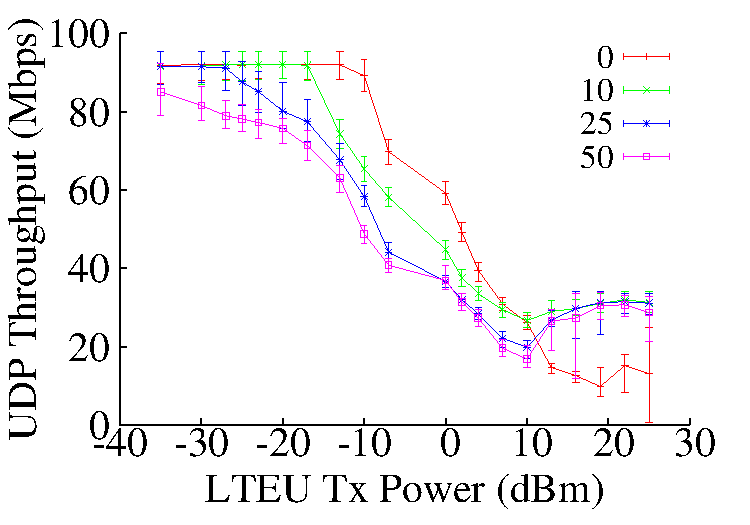
\includegraphics[width=3.0in, angle=0]{./figures/impact_nrbs_tplink} 
         \vspace{-0.0cm}
         \caption{The impact of RBs on commercial router.}         
        \label{impact_nrbs:a}
    \end{subfigure} %

    \begin{subfigure}[b]{\linewidth} \centering 
     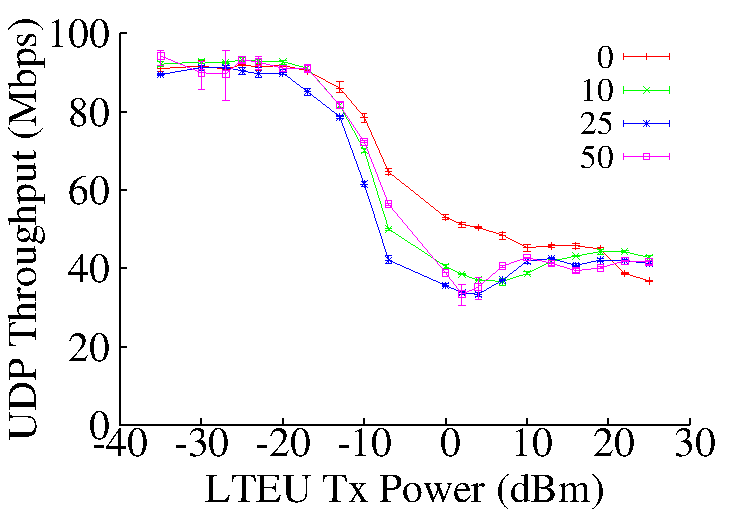
\includegraphics[width=3.0in, angle=0]{./figures/impact_nrbs_openwrt}  
        \vspace{-0.0cm}
        \caption{The impact of RBs on OpenWRT router.}
        \label{impact_nrbs:b}    
    \end{subfigure} 
\caption{The impact of RBs.}
\label{impact_nrbs}
\vspace{-0.2cm}
\end{figure}





\subsection{Increased Latency}

We evaluate the Wi-Fi latency by using ping command
when the duty cycle is 50\%. 
The received LTE-U power is higher than the 
energy detection threshold. 
We fix the duty cycle to be 50\% and use different
``on'' period, i.e., 5ms, 10ms, and 20ms.
As the baseline, we also measure the round trip time
when there is no LTE-U transmission.  
As can be seen in Fig. \ref{fig:impact_latency},
the round trip time of Wi-Fi link is less
than 2ms in more than 90\% of the time.  
Half of the Wi-Fi packets experience 
more than 5ms latency when the
``on'' period is 5ms.
This is because the packets are buffered and
waited to be transmitted until the channel is
clear. 
Increased ``on'' period reduces the latency
of most Wi-Fi packets, but increases
the tail latency.  

\begin{figure}[!ht]
 \centering
    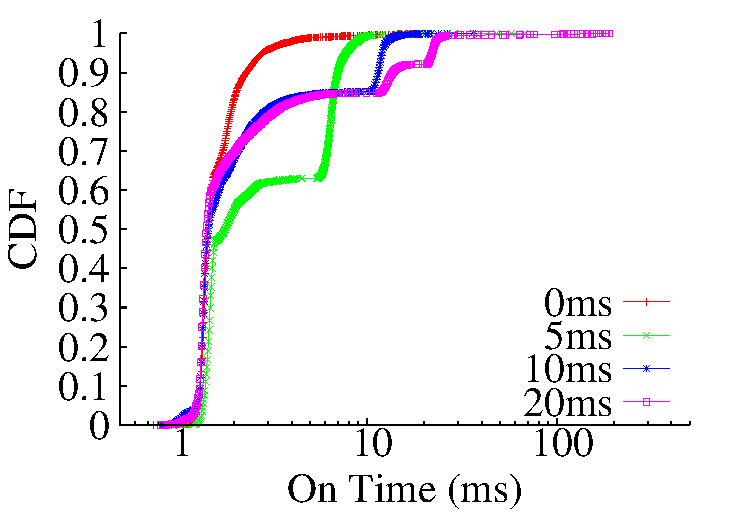
\includegraphics[width=3.0in]{./figures/impact_latency_ontime}
 \caption{Latency under different ``on'' period with 50\% dutcy cycle.}
  \label{fig:impact_latency}
\end{figure}


\subsection {Results Summary}

\begin{itemize}

\item Different routers, with different sensing and 
rate adaptation algorithms, show different coexistence 
capability under the interference of LTE-U. 
In our measurement, OpenWRT router performs best and is able
to better coexist with LTE-U under symmetric link settings, 
DD-WRT and commercial routers are affected by LTE-U
intereference under various received power and duty cycles. 
 

\item Since the starting of the LTE-U ``on'' period may kill Wi-Fi packet 
  in the air, longer LTE-U on time has less impact on WiFi UDP throughput, while
has higher impact on latency.  


\item The number of resource blocks in LTE-U frames has different impacts on WiFi UDP throughput, 
Less occupied frames are using less power than fully occupied frames, 
which makes WiFi may fail to sense the transmission of LTE-U. 


\end{itemize}





